\chapter{Lecture Notes}
\setlength{\headheight}{12.71342pt}
\addtolength{\topmargin}{-0.71342pt}

\section{04.09.24 - Microscope}

\subsection{Parts of the microscope}
The Microscope is put together by different components, as shown in Figure \ref{fig:MicroscopeComponents}. 

\begin{figure}[h]
    \centering
    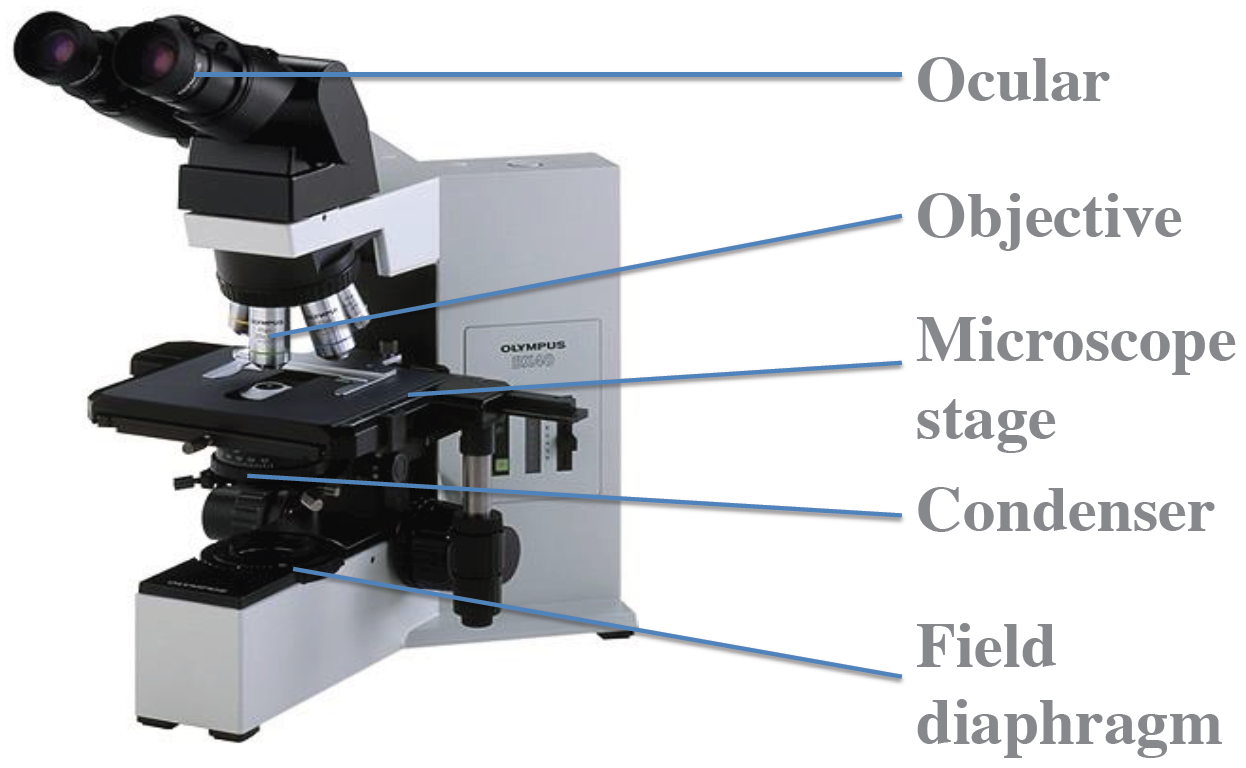
\includegraphics[width=0.45\textwidth]{Figures/MicroscopeComponents.png}
    \caption{The different components of a microscope.}
    \label{fig:MicroscopeComponents}
\end{figure}

The main components are: 
\begin{highlight}
    \begin{itemize}

        \item Ocular
        \subitem This is the set of lenses that you peer into, when you use a microscope. The “only” purpose of this part is to relay the intermediate image created by the objective to the retina of our eyes, i.e. to make us see an image. The ocular also magnifies the intermediate image with the factor of the ocular (usually around 10x); however, increasing the magnification of the ocular does not increase the resolving power (finer details of the specimen will not be 
        revealed)

        \vspace{5pt}\hrule\vspace{5pt}

        \item Objective
        \subitem Resolves the structure of the specimen, creating an intermediate image inside the microscope. The image is magnified with the factor depicted on the objective (often 10X, 40X and 100X). The objectives can be changed by rotating the objective turret, but this must be done cautiously to avoid mechanical damage. Objectives fitted for phase contrast will also be labelled with the size of the phase ring (usually this is depicted on the objective as either PH1, PH2 or PH3)

\end{itemize}
\end{highlight}

\begin{highlight}
    \begin{itemize}

        \item Microscope stage
        \subitem The (translation) microscope stage holds the specimen firmly with a specimen holder, and allows the specimen to be moved in fine increments in two dimensions

        \vspace{5pt}\hrule\vspace{5pt}

        \item Condenser
        \subitem * The condenser is located underneath the
        microscope stage. The purpose of this optical part is to illuminate our specimen optimally
        
        \subitem * Our microscopes for microbiological work have a condenser with a rotating turret that enables the use of phase contrast imaging, as a specific annular ring in this turret must be matched with the size of the phase ring in the objective. There is a cut-out on the front of the turret that depict the actual selection. In this picture the Ph2 ring has been selected
    
        \subitem * Apart from the phase rings, the turret also includes a blank opening that allows for traditional brightfield observation depicted with a 0, and a setting for darkfield depicted with a DF

    \end{itemize}
\end{highlight}

\subsection{Contrast methods}

\subsubsection*{Brightfield}
This simply magnifies the specimen. However it is almost impossible to see cells, without a staining procedure, that selectively  stains parts of the cells. Quite often, a stained specimen is also fixed, which means that the cells have been killed, so for live specimens (e.g. live bacteria), we need a different contrast method.

\subsubsection*{Darkfield}
This is only useful for 10X objectives or smaller, so for 
observing virtually all living cells.

\subsubsection*{Phase contrast}
This is the best method. The theory behind phase contrast is a little complicated (but hey - the guy won the Nobel Prize), but you can utilize phase contrast without knowing the theory. All you have to remember is:

\begin{highlight}
    \begin{itemize}
        \item The number on the phase objective and the number on the condenser turret must match to obtain a proper image (e.g. Ph 2 for the 40 x objective)
        \item The Field diaphragm in the bottom of the microscope should be completely open
    \end{itemize}
\end{highlight}

\subsection{How to use the microscope}

\subsubsection*{Preparing the microscope}
Set the ocular distance to match YOUR interpupillary distance; The distance between the eyes of people differs a lot. Our microscopes are equipped with two eyepieces, in order for you to look down the microscope in the same way as you look through a binocular, and ultimately the same way as you look on the world as such. Therefore, the first thing to do when you approach a microscope is to adjust the ocular distance to your individual interpupillary distance. The ocular distance can be read on a mm-scale (commonly 50-75) between the oculars.

The interpupillary distance is extremely easy to obtain, because you simply ask a friend to measure the distance between your pupils with an ordinary ruler. Memorise this value (because it is the same for the rest of your life), and adjust the oculars to your distance before you do anything else. This increases the comfort of using a microscope tremendously.

\section{04.09.24 - Yeast: Cytology, taxonomy and physiology}

\subsection{Background}
Yeast are quite different from bacterias, first of all, they are bigger than bacterias. Yeast are also eukaryotic, which means that they have a nucleus, and they have a lot of organelles. The yeast \textit{Saccharomyces cerevisiase} has a pair of 16 chromosomes, which is quite a lot for a yeast and thus making it a non-haploid.
The many differences from bacteria will influence their identification, their growth characteristics as well as the interactions with the food matrix. Proper identfication of yeast is therefore important for the correct use of starter cultures as well as for spoilage yeasts.

\subsection{Eukaryotes}

Since yeast are Eukaryotes, here are some key features of Eukaryotes:
\begin{highlight}
    \begin{itemize}
        \item Eukaryotes contain far more DNA than prokaryotes (x 100-1000). Yeast genome sizes
        range from 10-15 Mb and encode 5000-10000 genes
        \item The DNA is organised in a number of chromosomes
        \item The chromosomes are organised in a nucleus
        \item The presence of mitochondria
        \item The presence of different organelles such as: the Golgi apparatus and the endoplasmic
        reticulum
        \item Besides partly being involved in killer toxin production, the function of plasmids in
        yeasts is not really known
    \end{itemize}
\end{highlight}

\subsection{Organelles}

\begin{highlight}
    \begin{itemize}
        \item \textbf{CW: Cell wall (physical protection, adhesion etc.)}
        \item P: Periplasm
        \item \textbf{CM: Plasma membrane (transport in/out of the cytoplasma)}
        \item CMI: Invagination
        \item BS: Bud scar
        \item C: Cytoplasm
        \item \textbf{N: Nucleus (DNA in chromosomes)}
        \item \textbf{M: Mitochondrion (ATP synthesis, enzymes)}
        \item S: Secretory vesicles
        \item \textbf{V: Vacuole (protein trafficking, storage)}
        \item PER: Peroxisome
        \item ER: Endoplasmic reticulum
        \item G: Golgi apparatus
    \end{itemize}
\end{highlight}

In this course, we will focus on the cell wall, the plasma membrane, the nucleus, the mitochondrion and the vacuole. Though the other listed organelles are important, they are not as important for the physiology of yeast.

\subsubsection*{Cell wall}
The cell wall gives the yeast physical protection against the environment. It also maintains the shape of the yeast cell, and it is important for the osmotic stability of the yeast cell. The cell wall also has permeability barriers, which means that solutes larger than 620-760 Da can not pass the cell wall. The cell wall also has enzyme support, cation binding, cell-cell recognition and adhesion to other surfaces.

\subsubsection*{Plasma membrane}
The primary functions of the yeast plasma membrane are to dictate what enters and what leaves the cytoplasma i.e. to be a primary barrier for passage of hydrophilic molecules and prevent cytoplasmic contents to mix with the environment. The plasma membrane is also important for the uptake of nutrients, the excretion of waste products, the maintenance of the cell shape and the cell wall, and the cell division.

\subsubsection*{Nucleus}

\subsection{Methodologies for species identification of yeast} 
There are various methods for species identification of yeast, including:
\begin{highlight}
    \begin{itemize}
        \item Micro- and macromorphological identification added phenotypic characterisation
        \item Sequencing of the D1/D2 domain of the 26S rRNA gene (> 99\% homology = belong to the same species)
        \item Sequencing of multiple genes
        \item Sequencing of the ITS region (mostly moulds and yeasts identified by metagenomics)
        \item Identification of protein patterns by MALDI-TOF MS
        \item Analysis of biomas by Fourier Transform Infrared Spectroscopy (FTIR)
        \item Others...
    \end{itemize}
\end{highlight}

\subsection{Yeast taxonomy}
The taxonomy of yeast is quite complex, but it is important to know the different levels of taxonomy. The taxonomy of yeast is as follows:
\begin{highlight}
    \begin{itemize}
        \item Kingdom: Fungi (Both yeast and moulds are fungi)
        \item \textbf{Phylum:} e.g Ascomycota // Basidiomycota
        \item \textbf{Class:} e.g \textit{Saccharomycetes}
        \item \textbf{Order:} e.g \textit{Saccharomycetales}
        \item Family: e.g \textit{Saccharomycetaceae}
        \item Genus: e.g \textit{Saccharomyces}
        \item Species: e.g \textit{Saccharomyces 
        cerevisiae}    

    \end{itemize}
\end{highlight}

The following is not universally recognized, but are used in some contexts:
\begin{highlight}
    \begin{itemize}
        \item Subspecies: e.g \textit{Saccharomyces cerevisiae} subsp. \textit{cerevisiae}
        \item Variety: e.g \textit{Saccharomyces cerevisiae} var. \textit{cerevisiae}
        \item Strain: e.g \textit{Saccharomyces cerevisiae} subsp. \textit{cerevisiae} strain \textit{S288C}
    \end{itemize}
\end{highlight}

\subsection{Substrates for yeasts}
Following are some examples of some substrates which are greatly used for the propagation of yeasts:

\begin{highlight}
    \begin{itemize}
        \item Malt yeast extract Glucose Peptone agar (MYGP)
        \item Yeast extract Peptone Glucose (YPG) agar
        \item Malt Agar (MA)
        \item Lysine agar a.o. (for non-Saccharomyces yeasts)
        \item WLN medium (allows separation by coloration)
        \item Others\dots
    \end{itemize}
\end{highlight}

There are som stress tolerant yeasts where high concentrations of substrates are needed in the media for the growth of specific yeast. Some examples of medias for stress tolerant yeasts can be seen in \ref{fig:StressTolerantYeasts}.

\begin{figure}[h]
    \centering
    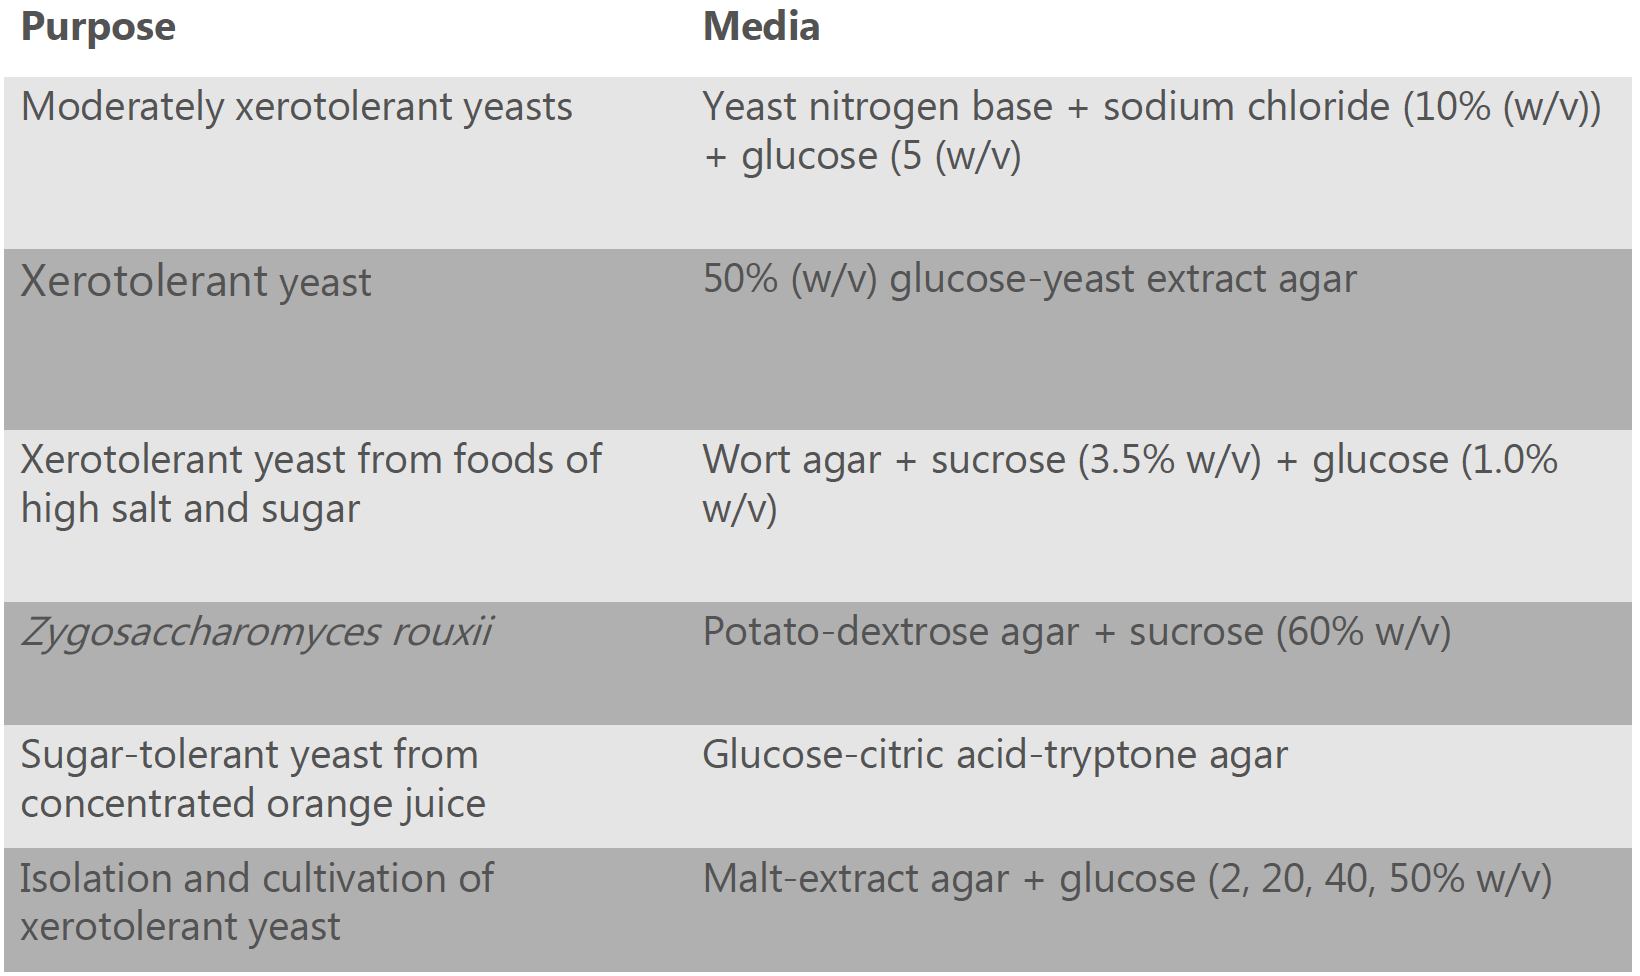
\includegraphics[width=1\textwidth]{Figures/StressTolerantYeast.png}
    \caption{Examples of medias for stress tolerant yeasts.}
    \label{fig:StressTolerantYeasts}
\end{figure}


\subsection{Conventional methods for identification of yeast}
There are various methods for identification of yeast, here are a list of some of the most common methods:
\begin{highlight}
    \begin{itemize}
        \item By their cultural characteristics
        \subitem Solid media: colony morphology, color, size, shape, surface, margin, elevation, texture
        \subitem Liquid media: turbidity, sediment, pellicle, ring, flocculation
        \item By their cell morphology and arrangement
        \subitem Cell form and size 
        \subitem Vegetative reproduction by budding or fission
        \subitem Pseudomycelium or true mycelium
        \item By their sexual characteristics
        \subitem Perfect stage (\textit{teleomorph}) or imperfect stage (\textit{anamorph})
        \subitem By their formation and arrangement of spores 
        \item Biochemical characteristics
        \subitem Assimilation of carbon or nitrate sources (e.g. API20c, ID32c)
        \subitem fermentation of carbohydrates
        \item Physical and chemical tolerance
        \subitem Growth in the presence of 100 or 1000 ppm cycloheximide
        \subitem Growth in the presence of 1\% acetic acid
        \subitem Growth on 50\% glucose-yeast extract agar
        \subitem Etc.
    \end{itemize}
\end{highlight}

\subsection{Macro-morphological characteristics}
There are many different macro-morphological characteristics of yeast, some of the ones we will be using in this course laboratory exercises can be seen in figure \ref{fig:Macromorp}.

\begin{figure}[h]
    \centering
    \rotatebox{90}{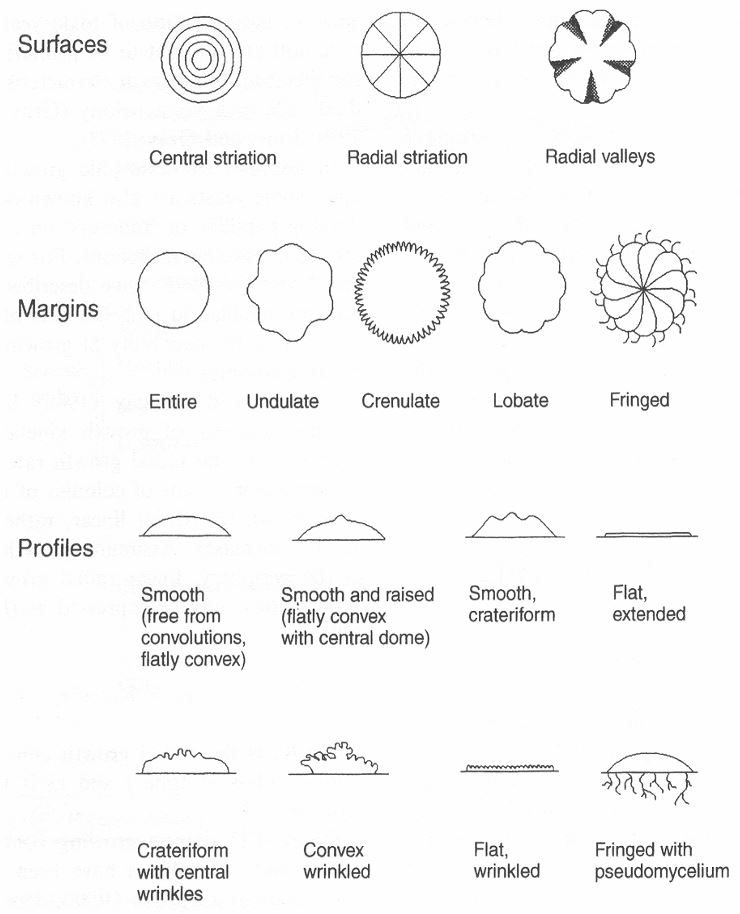
\includegraphics[width=0.55\textwidth]{Figures/Macromorph.JPG}}
    \caption{Examples of macro-morphological characteristics of yeast that will be evaluated in the laboratory exercises.}
    \label{fig:Macromorp}
\end{figure}

Furthermore, the lecture included a list of some key aspects to keep in mind while looking at the macro-morphological characteristics colonies. These are:
\begin{highlight}
    \begin{itemize}
        \item Tecture (mucoid, viscous, matted, coherent etc.)
        \item Color
        \item Size
        \item Surface (glistening, smooth, verrucose, rough etc.)
        \item Elevation
        \item Margin (entire, rhizoid etc.)
        \item Mycelium (x100 magnification)
    \end{itemize}
\end{highlight}

\subsection{Micro-morphological characteristics}
Micro-morphological characteristics are also important when identifying yeast. Some of the key aspects are listed below:

\begin{highlight}
    \begin{itemize}
        \item Cell form (spheroidal, ellipsoidal, ovoid, lemon-shaped, 
        elongated, triangular etc.)
        \item Cell size (length, width)
        \item Cell arrangement (pairs, aggregates)
        \item  Vegetative reproduction
        \subitem Budding (monopolar, bipolar, multilateral)
        \subitem Fission 
        \item Mycelium
        \subitem Pseudomycelium (not distint septa)
        \subitem True mycelium (distint septa)
    \end{itemize}
\end{highlight}

\subsection{Assimilation and fermentation}
Assimilation refers to the process by which an organisms takes in and incorporates nutrients from the environment. The assimilation of carbon compounds is important for the growth of yeast. Yeast assimilates carbon compounds by various pathways, like Krebs cycle (TCA pathway) or the glycolysis.

Fermentation is the process by which yeast converts sugars into alcohol and carbon dioxide. The fermentation of carbohydrates typically happens under anaerobic conditions. The fermentation process is a less efficient energy source than respiration. Nevertheless, without it, wine and beer could not be made. Brewers therefore exploit the yeasts fermentative capability by introducing yeast into an anaerobic environment. 

\subsubsection*{Assimilation of carbon compounds}
To propagate yeast while having assimilation in mind, the growth medium  Yeast Nitrogen Base from "Difco" can be used. This medium contains:

\begin{highlight}
    \begin{multicols}{3}
        \begin{itemize}
            \item Hexoses
            \item Trisaccharides
            \item Pentoses
            \item Organic acids
            \item Disaccharides
            \item Polysaccharides
            \item Alcohols
            \item Glycosides
        \end{itemize}
    \end{multicols}
\end{highlight}

\subsubsection*{Fermentation of carbon compounds}
Here are a list of some of the carbon compounds that yeast can ferment:

\begin{highlight}
    \begin{multicols}{3}
        \begin{itemize}
            \item Glucose
            \item Maltose
            \item Trehalose
            \item Galactose
            \item Raffinose
            \item Melibiose
            \item Saccharose
            \item Lactose
            \item Inulin
        \end{itemize}
    \end{multicols}
\end{highlight}

\subsubsection*{Assimilation of nitrogen compounds}
To propagate yeast while having assimilation in mind, the growth medium Yeast Carbon Base from "Difco" can be used. This medium contains:

\begin{highlight}
    \begin{multicols}{2}
        \begin{itemize}
            \item Nitrate
            \item Ethylamine hydrochloride
            \item L-lysine
            \item Creatine
            \item Nitrite
            \item Cadaverine dihydrochloride
            \item Creatinine
        \end{itemize}
    \end{multicols}
\end{highlight}

\subsection{Vegetative reproduction (genera)}
Vegetative reproduction is the process by which a plant or fungus reproduces asexually. Yeast can reproduce vegetatively by budding or fission. Some examples of yeast vegetative reproduction is:

\begin{highlight}
    \begin{multicols}{2}
        \noindent
        \textbf{Bipolar}
        \begin{itemize}
            \item \textit{Hanseniaspora (Kloeckera)}
            \item \textit{Rhodotorula}*
            \item \textit{Saccharomycodes}
            \item \textit{Trichosporon}
        \end{itemize}
        
        \vspace{1em}

        \textbf{Fission}
        \begin{itemize}
            \item \textit{Schizosaccharomyces}
        \end{itemize}
        
        \vspace{1em}

        \textbf{Arthroconidia}
        \begin{itemize}
            \item \textit{Galactomyces (Geotrichum)}
            \item \textit{Saccharomycopsis}*
        \end{itemize}
        
        \vspace{1em}

        \textbf{Enterobalstic Budding}
        \begin{itemize}
            \item \textit{Phaffia}
        \end{itemize}
        
        \columnbreak
        
        \textbf{Multilateral}
        \begin{itemize}
            \item \textit{Candida}
            \item \textit{Debaryomyces}
            \item \textit{Dekkera (Brettanomyces)}
            \item \textit{Kazachstania}
            \item \textit{Kluyveromyces}
            \item \textit{Pichia}
            \item \textit{Rhodotorula}*
            \item \textit{Saccharomyces}
            \item \textit{Saccharomycopsis}*
            \item \textit{Torulaspora}
            \item \textit{Yarrowia}
            \item \textit{Zygosaccharomyces}
        \end{itemize}
    \end{multicols}
\end{highlight}
*Two types of vegetative reproduction my be present

\subsection{Lecture conclusion}
\begin{highlight}
    \begin{itemize}
        \item Yeasts are predominantly unicellular eukaryotes
        \item Yeasts might have both imperfect and perfect names
        \item Yeast taxonomy is changing continuously especially due to new molecular 
        techniques 
        \item Yeasts are currently mostly identified by sequencing of the D1/D2 region of 
        the 26S rRNA gene – however, never forget to verify by examining 
        morphology and include phenotypic tests
        \item Remember to consult the newest scientific literature in order to use up
        dated taxonomic names
    \end{itemize}
\end{highlight}

\section{09.09.24 - Taxonomy and the species concept}

\subsection{Lecture content}

During this lecture the following topics will be the focus point.

\begin{highlight}
    \begin{itemize}
        \item Definitions of taxonomy and phylogeny
        \item Phylogeny
        \item Microbial taxonomy: from domain to species
        \subitem Species concept in Bacteria
        \subitem Species concept in Yeast and Moulds
        \item Subspecies, variant and strains
    \end{itemize}
\end{highlight}

\subsection{Taxonomy and phylogeny}
From figure \ref*{fig:TaxDiff} we can see that the common ancestor of Bacteria, Archaea and Eukaryota is the root of the tree, and the branches of the three domains is what sums up the tree. 
\begin{figure}[h]
    \centering
    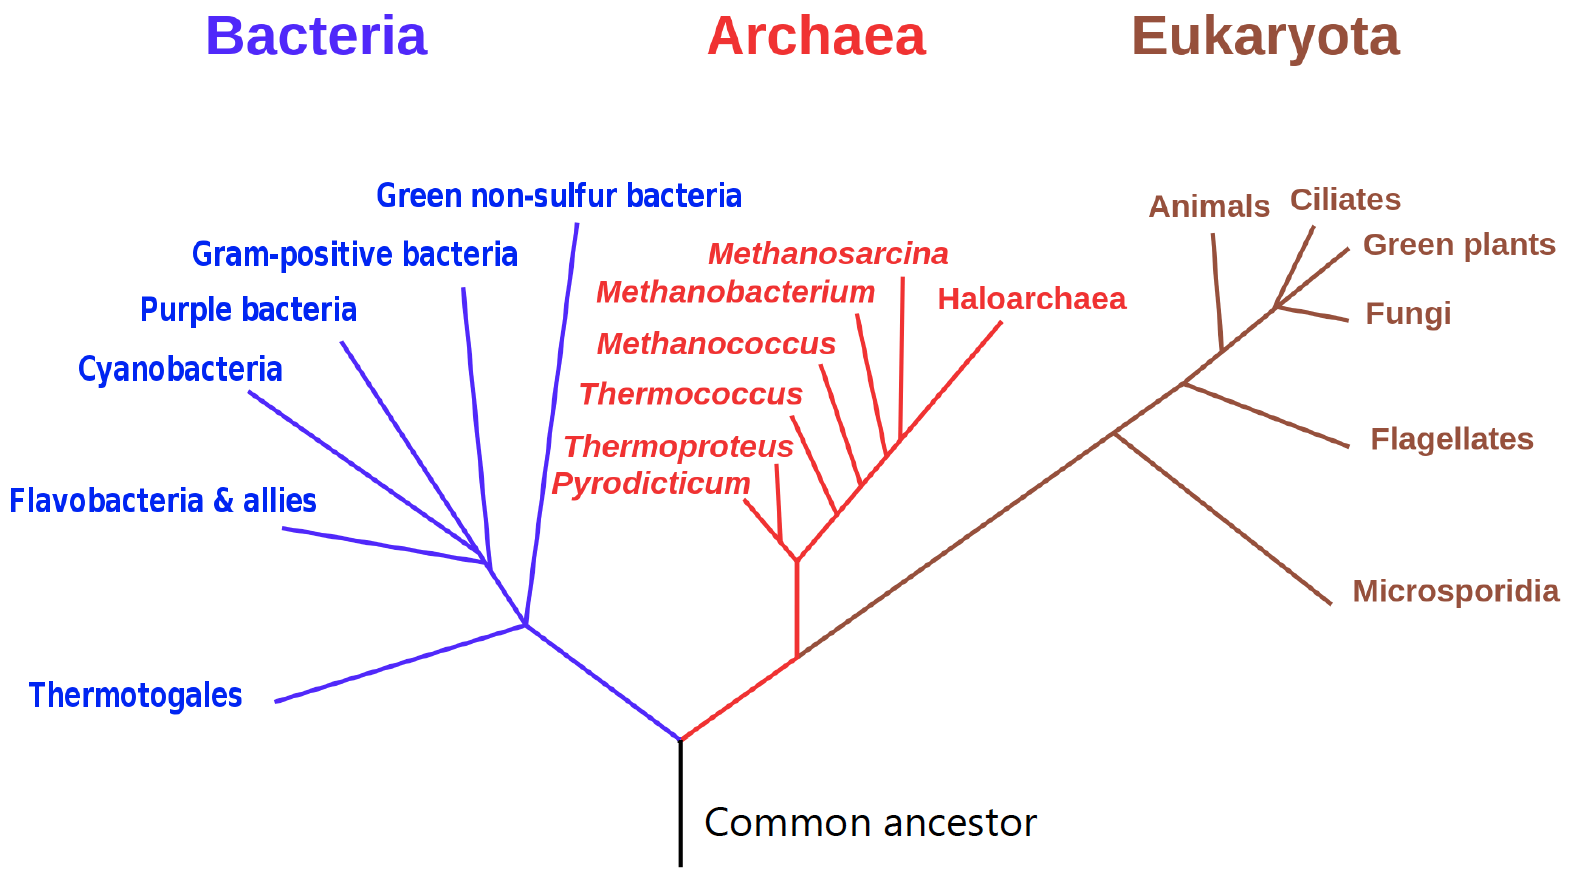
\includegraphics[width=0.72\textwidth]{Figures/TaxonomyDiff.png}
    \caption{The comon ancestor of Bacteria, Archaea and Eukaryota and the som of their respective branches}    \label{fig:TaxDiff}
\end{figure}

A definition \textbf{Taxonomy}, this the naming and classification of organisms based on shared properties, which can be based on

\begin{highlight}
    \begin{itemize}
        \item Genotypic properties
        \item phenotypic properties
        \item Phylogeny - evolutionary relationships
    \end{itemize}
\end{highlight}

While working with taxonomy and phylogeny in a broder sense, some of the following terms are important to know:

\begin{highlight}
    \begin{itemize}
        \item \textbf{Isolation:} The separation of a pure culture from a mixed culture
        \subitem \textbf{Sampling:} The collection of a representative part of a population
        \subitem \textbf{Colony purification:} The isolation of a single colony from a mixed culture
        \subitem \textbf{DNA extraction:} The isolation of DNA from a pure culture
        \item \textbf{Identification:} The determination of the taxonomic position of an organism
        \subitem \textbf{Microscopy:} The determination of the morphology of an organism through a microscope
        \subitem \textbf{Sequencing:} The determination of the sequence of a gene or a genome
    \end{itemize}
\end{highlight}

While looking at the phylogeny we can look deeper into the classification, in table \ref*{tab:ClassificationPhylogeny} we can see an example of the classification of a Bacteria and Eukarya where we stop at species. This can be further divided into subspecies, variant and strains.

\begin{table}[h]
    \centering
    \caption{An example of the classification of a Bacteria and Eukarya}
    \label{tab:ClassificationPhylogeny}
    \begin{tabular}{c|c|c}
        Domain & Bacteria & Eukarya \\
        Kingdom & None assigned & Fungi \\
        Phylym & Firmicutes & Ascomycota \\
        Class & Bacilli & Saccharomycetes \\
        Order & Lactobacillales & Saccharomycetales \\
        Family & Lactobacillaceae & Saccharomycetaceae \\
        Genus & \textit{Lactobacillus} & \textit{Saccharomyces} \\
        Species & \textit{L. acidophilus} & \textit{S. cerevisiae} \\
    \end{tabular}    
\end{table}

In the following table, there will be listed some differences between prokaryotes and eukaryotes.

\begin{table}[h]
    \centering
    \caption{Differences between prokaryotes and eukaryotes}
    \label{tab:DiffProkEuk}
    \begin{tabular}{c|l|l}
        & \textbf{Prokaryotes} & \textbf{Eukaryotes} \\
        \hline
         & 
        DNA is naked & DNA is bound to protein \\
        \textbf{DNA} & DNA is circular & DNA is linear \\
        & Usually no introns & Usually has introns \\
        \hline
        & No nucleus & Has a nucleus \\
        \textbf{Organelles} & No membrane-bound & Membrane-bound \\
        & 70S robossoms & 80S ribosomes \\
        \hline
        \textbf{Reproduction} & Binary fission & Mitosis \& meiosis \\
        & Single chromosomes (haploid) & Chromosomes paired (diploid or more)\\
        \hline
        \textbf{Average size} & Smaller (~1-5 $\mu$m) & Larger (~10-100 $\mu$m) \\
    \end{tabular}
\end{table}

\subsection{Gram-positive \& -negative bacteria}
(Almost) all bacteria can be divided into two groups, Gram-positive and Gram-negative bacteria. The difference between the two groups is the cell wall. The cell wall protects the bacteria e.g against osmotic stress. The cell wall differs where the Gram-positive bacteria have a thick cell wall, while the Gram-negative bacteria have a thin cell wall. The difference in the cell wall is due to the peptidoglycan layer, which is thicker in the Gram-positive bacteria than in the Gram-negative bacteria. The peptidoglycan layer is also the reason why the Gram-positive bacteria are more resistant to antibiotics than the Gram-negative bacteria. Here are some bulletpoints of the two groups:

\begin{highlight}
    \begin{itemize}
        \item \textbf{Gram-positive bacteria} 
        \subitem Lactic Acid Bacteria (LAB)
        \subitem Bacillus
        \item \textbf{Gram-negative bacteria}
        \subitem Most Acetic Acid Bacteria (AAB)    
    \end{itemize}
\end{highlight}

\subsection{Differentiating between bacterial species}
There are several methods to differentiate between bacterial species, some of the most common methods are:

\begin{highlight}
    \begin{itemize}
        \item \textbf{DNA:DNA hybridization (DDH)}: 
        \subitem The DNA of two organisms is mixed and the degree of hybridization is measured. 
        \subitem If DDH > 70\% the organisms are considered to belong to the same species
        \item \textbf{16S rRNA gene sequencing}:
        \subitem The 16S rRNA gene is sequenced and compared to a database, if the sequence is > 97.5-98.5\% 
        \subitem identical to a known species, the organism is considered to belong to the same species
        \item \textbf{Whole genome sequencing}:
        \subitem Average nucleotide identity (ANI) > 95-96\% is considered to belong to the same species
        \subitem Digital DNA-DNA hybridization (dDDH) > 70\% is considered to belong to the same species
    \end{itemize}
\end{highlight}

\section{11.09.24 - Methodologies for identification and typing}

\subsection{Intended leaning outcomes}

After this lecture, the students should be able to:
\begin{highlight}
    \begin{itemize}
        \item Get to know how different microbial identification and typing methods works
        \item Apply this knowledge to comprehend microbial identification and taxonomy
        \item Reflect on the application possibilities of the different methods for microbial identification and typing
    \end{itemize}
\end{highlight}

\subsection{Background}

\begin{highlight}
    \begin{itemize}
        \item When you want to know what microorganisms are in a fermented food
        \subitem \textbf{IDENTIFICATION}
        \item Often identification is coupled with quantification (predominant/minor microorganisms)
        \item Many different methods are available
        \subitem Make an overview of the most used methods
        \subitem Elaborate the steps of the methods → insights into the structure/mechanistics
        \subitem Show how the methods are applied
        \item All methods have strengths and limitations
    \end{itemize}
\end{highlight}

Note: typing is identification of isolates below species level

\subsection{Methodology overview}

\subsubsection*{Culture dependent methods}
This is the most common method for identification of microorganisms. The method is based on the growth of the microorganisms on a solid or liquid medium. Here are an example of a method which is based on this:
\begin{highlight}
    \begin{itemize}
        \item Plating
        \item Isolation
        \item Purification (The next 4 steps are methods for identification)
        \item Finger print based\textsuperscript{1}
        \subitem rep-PCR, RAPD, RFLP or PFGE (All these are based on PCR)
        \item Sequence based\textsuperscript{2}
        \subitem rRNA gene, MLST or MLSA
        \item Biochemical identification\textsuperscript{3}
        \subitem MALDI-TOF or FTIR
        \item Classical\textsuperscript{4}
        \subitem Macro/micro morphology, phenotypic tests (fermentation, assimilation or growth condi-
        \subitem tions)
    \end{itemize}
\end{highlight}



\subsubsection*{Culture independent methods}

\begin{highlight}
    \begin{itemize}
        \item Direct extraction of DNA or RNA
        \item Molecular methods (the next two steps are both molecular methods methods) 
        \item PCR\textsuperscript{1}
        \subitem Species specific PCR
        \item qRT-PCR\textsuperscript{2}
        \subitem Next generation sequencing
    \end{itemize}
\end{highlight}

\section{16.09 - From 1\texorpdfstring{\textsuperscript{st}}{st} to 3\texorpdfstring{\textsuperscript{rd}}{rd} generation DNA sequencing strategies}

DNA is quite small, 2 nm thick. Though, if folded out, the DNA would be around 1.8 m long. 


\subsection{Sanger Sequencing of DNA 1\texorpdfstring{\textsuperscript{st}}{st} generation sequencing}

\textcolor{blue}{5'- TACAACTGAGCGACT -3'}

3'- ATGTTGACTCGCTGA -5'

Here we have a blue sequence and a black complimenting sequence. If we want to sequence the blue sequence, we can use the black sequence as a primer. The primer will bind to the blue sequence, and the DNA polymerase will start to build a new strand of DNA. The DNA polymerase will build the new strand by adding nucleotides to the 3' end of the primer. The nucleotides are added in a 5' to 3' direction. The DNA polymerase will continue to add nucleotides until it reaches the end of the DNA strand. The DNA polymerase will then stop, and we will have a new strand of DNA. 

Though with the Sanger sequencing, we will have a mix of DNA strands, where each strand will end with a different nucleotide. The DNA strands will then be separated by size, and the sequence can be read by the size of the DNA strands.

With Sanger sequencing, the -A, -C, -G and -T nucleotides will cut the DNA strand at different lengths, because it cuts at the respective letter. An example of how the Sanger sequencing works can be seen in figure \ref{fig:SangerSequencing}.

\begin{figure}[h]
    \centering
    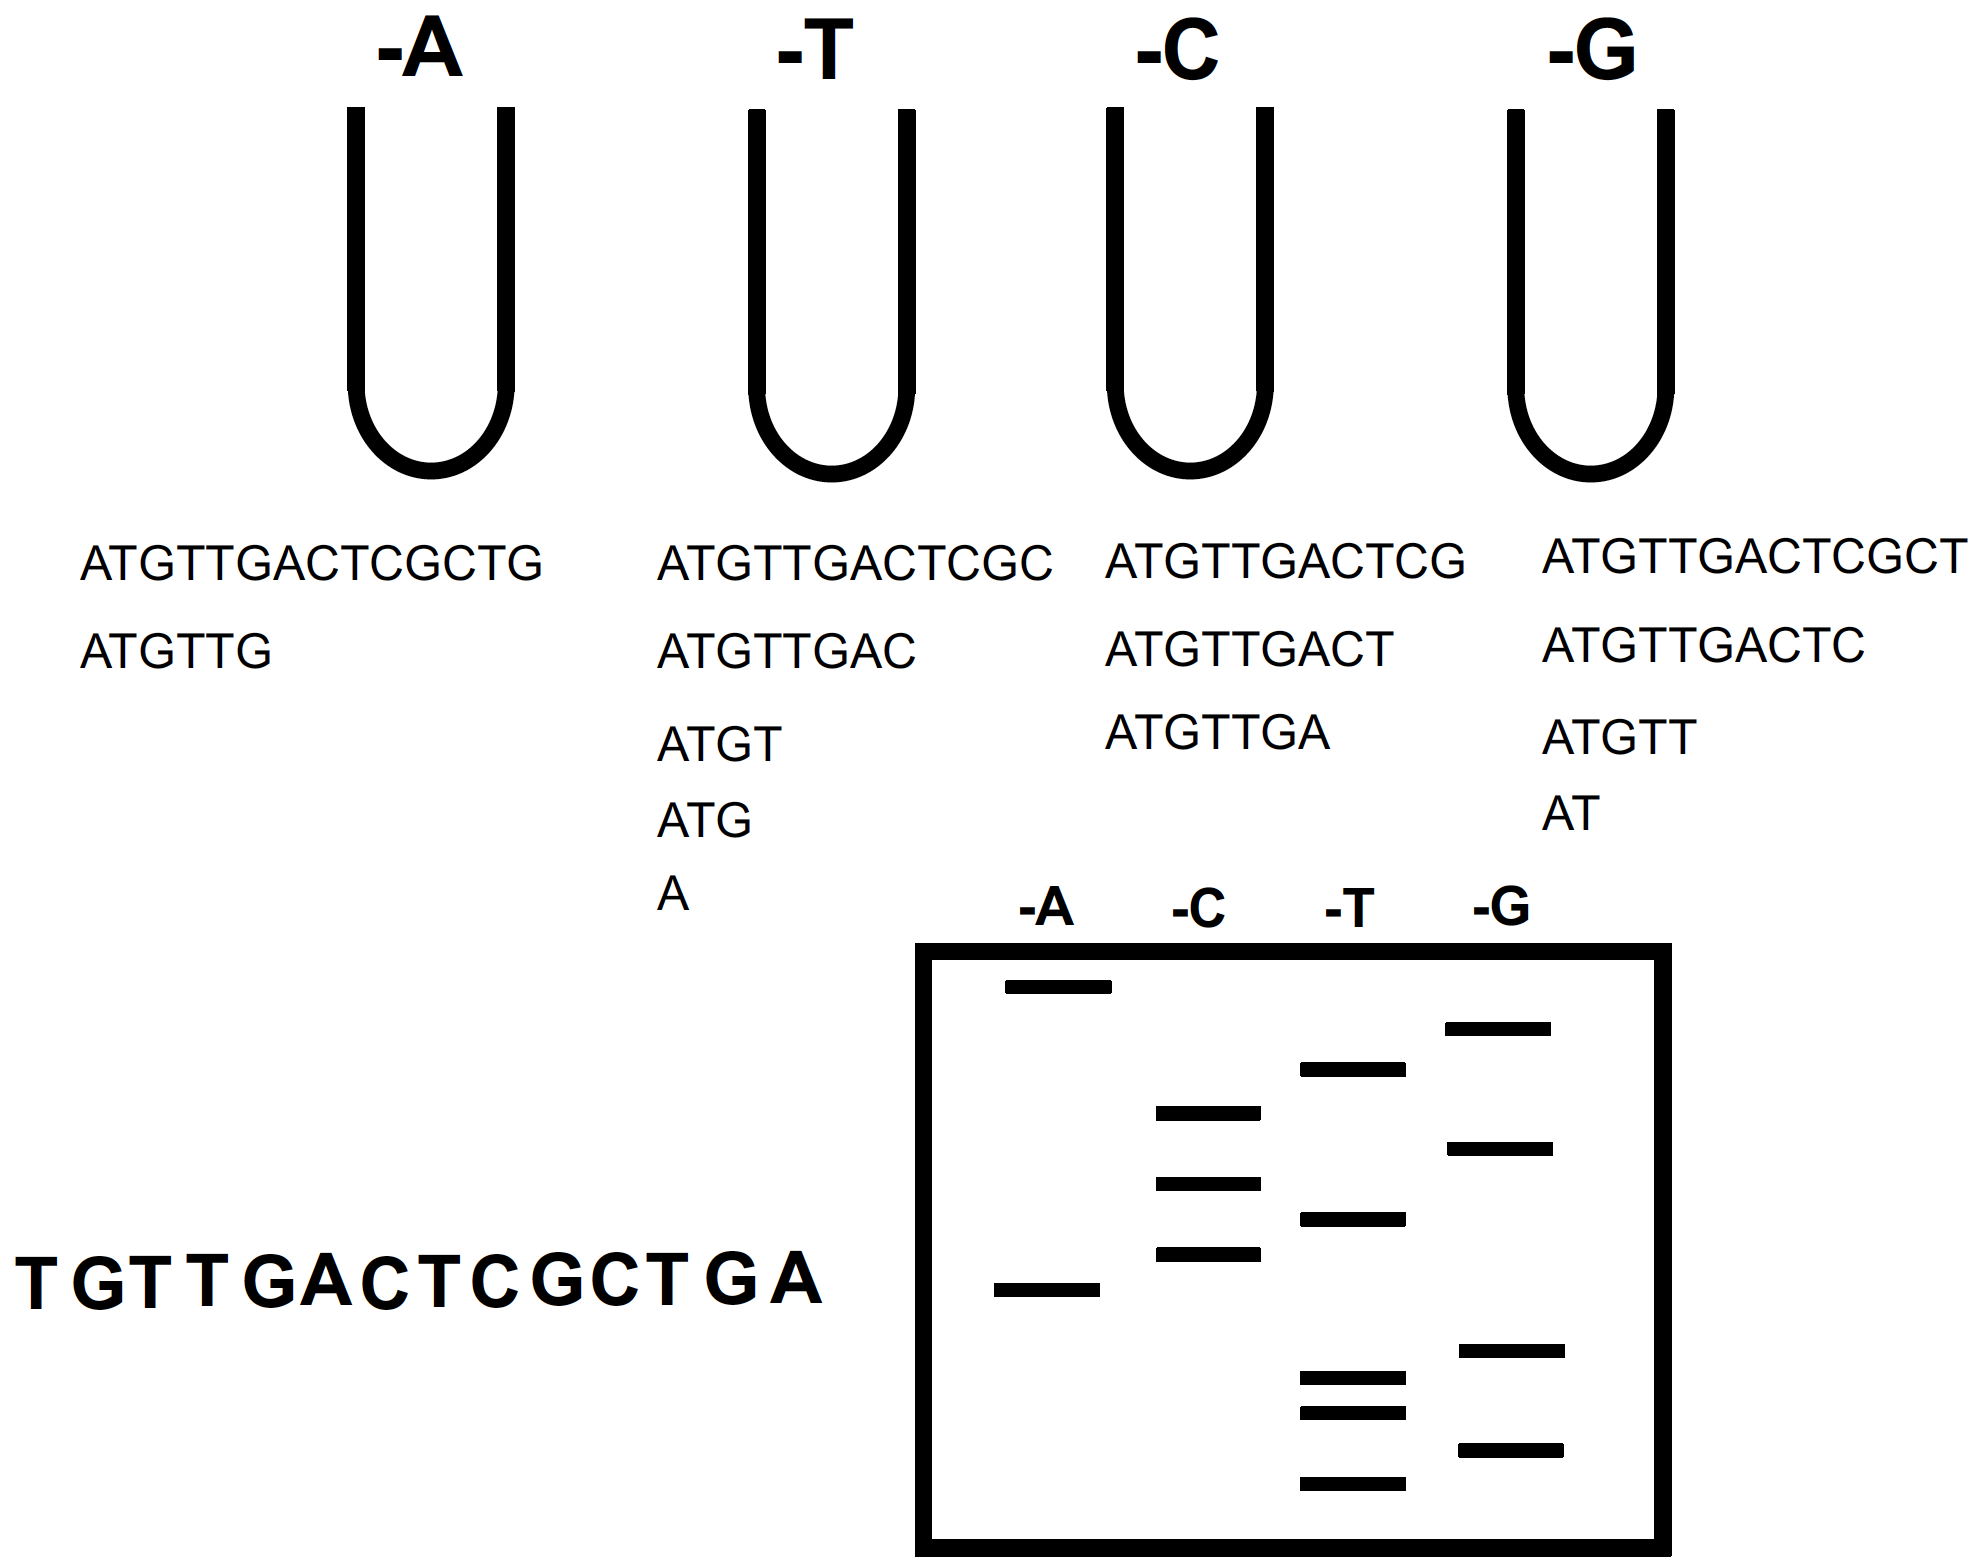
\includegraphics[width=0.7\textwidth]{Figures/SangerExample.png}
    \caption{An example of how the method of Sanger sequencing of DNA works with the given blue sequence}
    \label{fig:SangerSequencing}
\end{figure}



\subsection{Next generation sequencing}
Next generation sequencing (NGS), has been evolving a lot since extensive research started in the 90's. Today we have a lot of different NGS methods, one of the most common methods is the Illumina sequencing. The Illumina sequencing is based on the Sanger sequencing, but with a few modifications. Their HiSeqX can sequence around 50 human genomes in a day with a cost sub 1000 USD/genome.

\subsubsection{Sequencing by synthesis}
The Illumina sequencing is based on the sequencing by synthesis. It needs a primer, but these a fairly simple to make. 
After the primer has been added, the DNA polymerase will start to build a new strand of DNA. The DNA polymerase will add nucleotides from -A, -T, -G, anc -C, to the 3' end of the primer, and the nucleotides will be added in a 5' to 3' direction. The DNA polymerase will continue the flashing with nuclouetides until it reaches the end of the DNA strand. The DNA polymerase will then stop, and we will have a new strand of DNA. 

The maximum read out length of the Illumina is between 75 bp to 350 bp, but the average read length is around 150 bp.

\subsubsection{Bridge amplification}
A piece of DNA is attached to a glass slide, and the DNA is then amplified. The DNA is then denatured, and the DNA is then amplified again. The DNA is then denatured again, and the DNA is then amplified again. This process is repeated until the DNA is amplified enough. The DNA is then sequenced, and the sequence is read by the computer. This method grows exponentially like PCR, though the DNA is amplified in a half circle, and not in a straight line.

An example of how the Illumina bridge amplification works can be seen in figure \ref{fig:BridgeAmpl}.

\begin{figure}[h]
    \centering
    \begin{subfigure}{0.35\textwidth}
        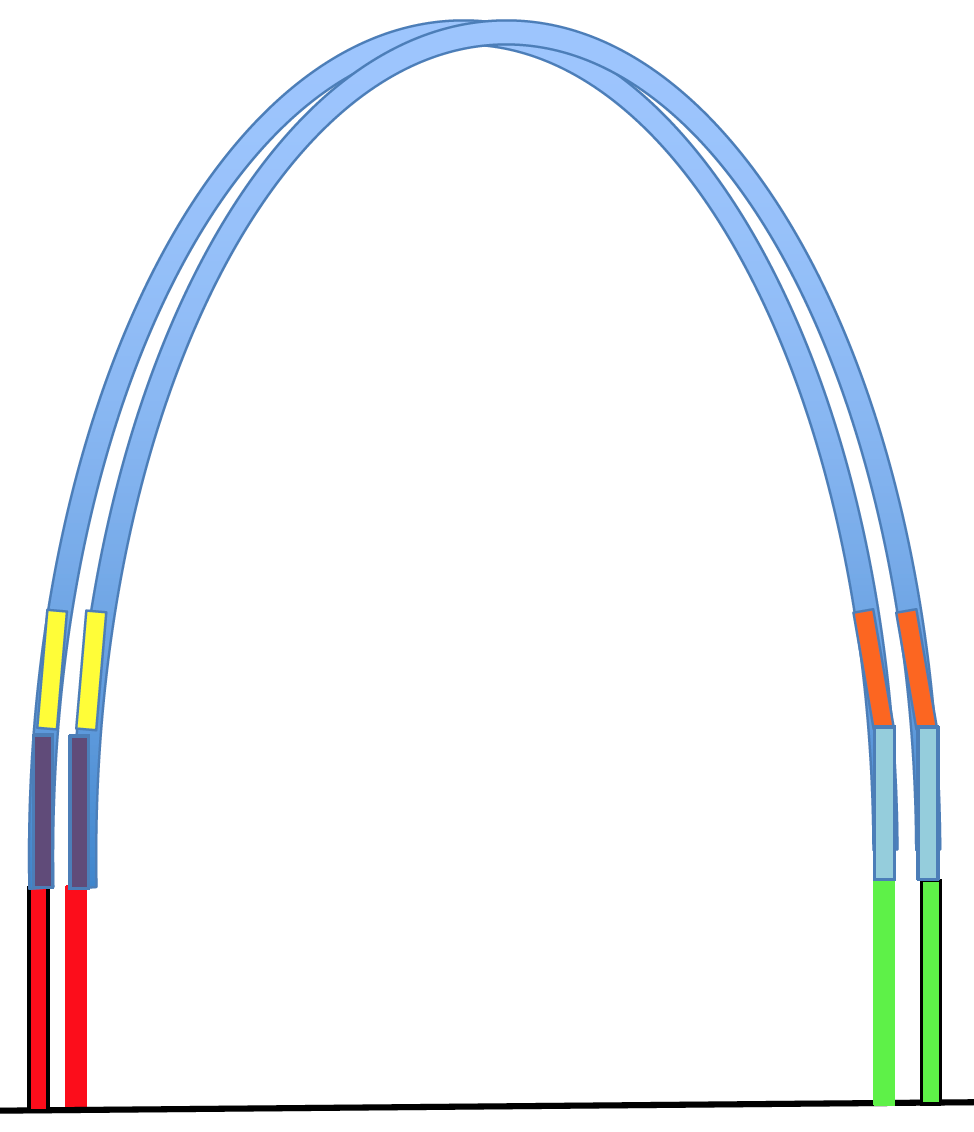
\includegraphics[width=\linewidth]{Figures/Bridge1.png}
        \caption{CHere an example of how the DNA is attached to the glass slide on both ends forming the bridge.}
    \end{subfigure}
    \hfill
    \begin{subfigure}{0.55\textwidth}
        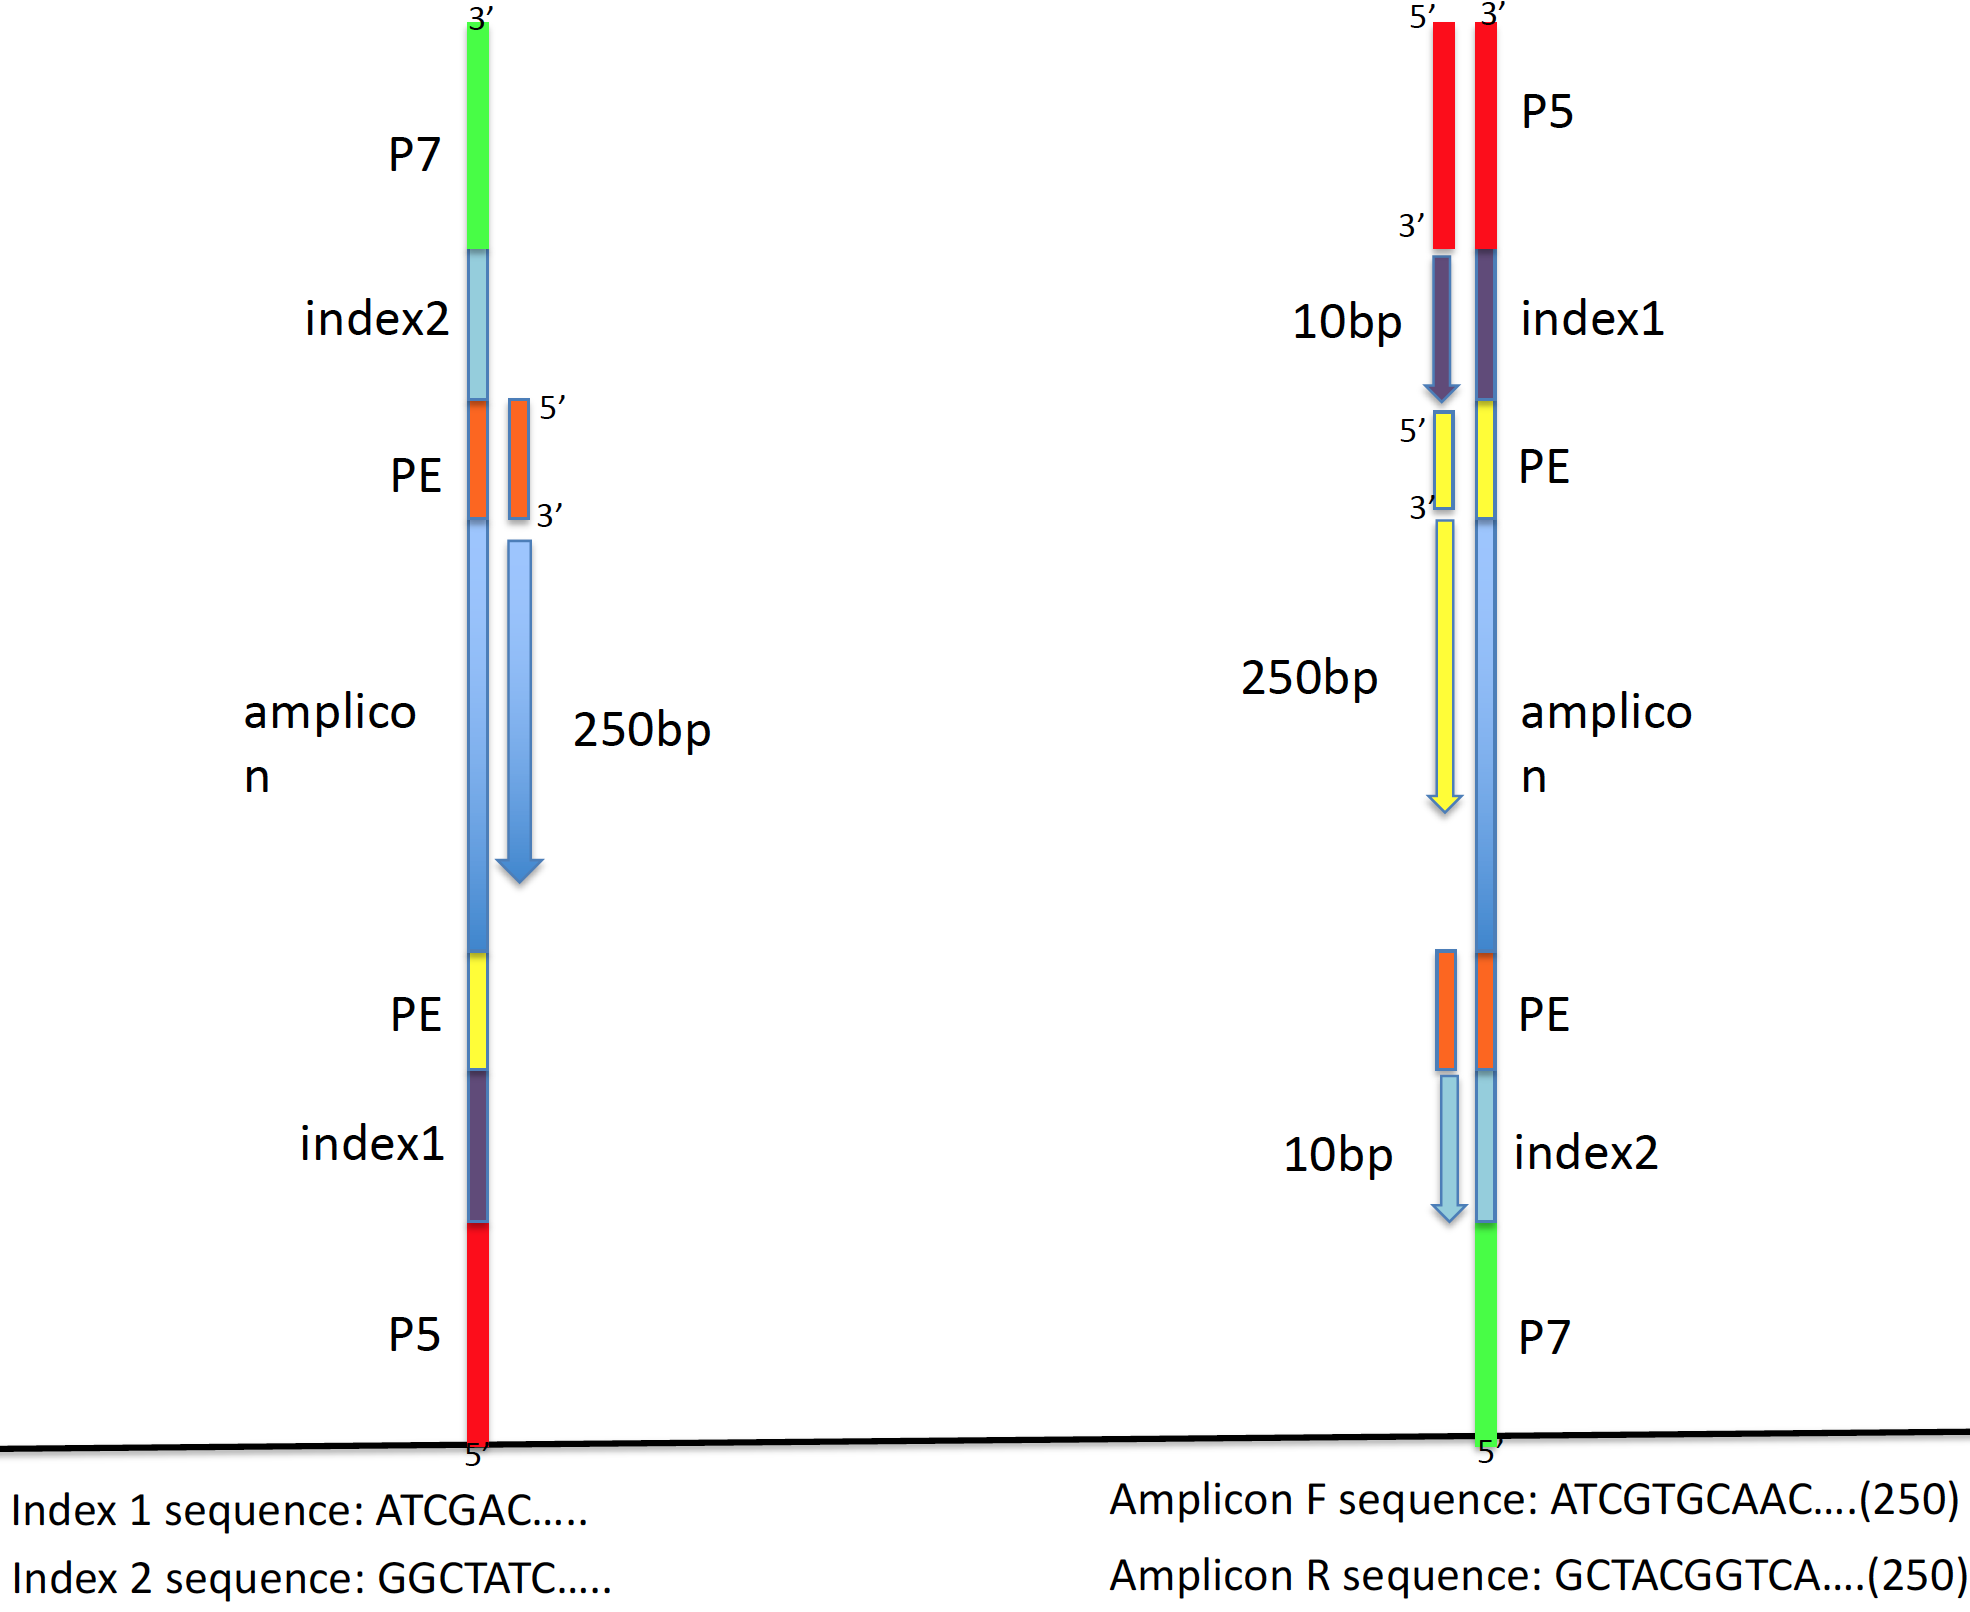
\includegraphics[width=\linewidth]{Figures/Bridge2.png}
        \caption{After heating the bridge opens up and the DNA is amplified.}
    \end{subfigure}
    \caption{An example of how the Illumina bridge amplification works.}
    \label{fig:BridgeAmpl}
\end{figure}

\subsection{3\texorpdfstring{\textsuperscript{rd}}{rd} generation sequencing}
Third-generation sequencing detects nucleotide sequences by measuring changes in ion flow across a membrane as molecules pass through a nanopore. Each nucleotide creates a distinct current profile, enabling identification of both type and sequence order \cite*{L5-HighThroughput}.

\section{18.09.24 - Moulds and their role in fermented food and beverages}
Moulds are utilized globally in the production of various food and beverages, offering unique functionalities and enzyme production capabilities.

\begin{itemize}
    \item You should be able to know the basic technological properties of moulds for use in the food and beverage industry
    \item You should be able to explain the basic of moulds taxonomy
    \item You should have a broad knowledge on the use of moulds in various products around the world and to be able to make idea generation on new innovative products
\end{itemize}
\subsection*{Background}
Moulds serve important roles in food production, providing enzymatic degradation of raw materials and contributing to flavour, texture, and color, while also posing risks due to mycotoxin production.

\subsubsection*{Moulds (snapshot)}
Moulds are eukaryotic multicellular organisms made of hyphae and produce spores, called conidia when imperfect.

\subsubsubsection*{Identification of Moulds}
Identification relies on the micro-morphology of conidia and spores, which are key taxonomic characteristics.

Growth on specific media can assist in identifying mould species based on their growth patterns.

Secondary metabolites can be profiled using HPLC to aid in identification.

Sequencing techniques, such as ITS or 28S, are valid methods for identifying moulds. 

\subsection*{Moulds as Enzyme Producers} 
Moulds are known for producing various enzymes that facilitate the transformation of substrates in food processing. Key enzymes include amylases, cellulases, pectinases, and proteases, each serving specific functions in food production.

Moulds are involved in the fermentation of various food types, both solid, liquid and semi-solid. They ferment through different patterns and use various substrates.

\subsection*{Mould-Ripened Cheeses}
Examples include Brie and Camembert, which rely on specific moulds for their unique properties.

\subsubsection*{Production of Danablu}
The growth phases of \textit{P. roqueforti} in Danablu cheese include germination, mycelial growth, and sporulation.

\subsubsection*{Remarks on Moulds in Cheese}
Different moulds produce distinct cheese types; environmental factors influence mould growth and cheese maturation.

\subsection*{Fermented Meat}
Moulds play a critical role in the fermentation of meat products, enhancing flavour and safety.

Moulds contribute to flavour development, color stabilization, and texture improvement in fermented sausages.

\subsection*{Noble Rot - Botrytis spp.} 
Botrytis cinerea induces noble rot in grapes, enhancing sugar concentration for wine production.

\subsection*{Quorn - Mycoprotein from Moulds} 
Quorn is produced from \textit{Fusarium venenatum}, cultivated in controlled conditions to create a meat substitute.

\subsection*{Examples of Mould Fermented Foods in Asia and Latin America}

\subsubsection*{Koji - An Inoculum}
Koji, made from \textit{Aspergillus oryzae}, is essential for saccharification (starch to glucose) in Japanese fermented foods.

\subsubsection*{Miso}
Miso is produced by fermenting soybeans with koji, resulting in a staple ingredient in Japanese cuisine.

\subsubsection*{Soy Sauce}
Soy sauce production involves fermentation with \textit{Aspergillus} species, enhancing flavour and aroma.

\subsubsection*{Tempeh}
Tempeh is made from fermented soybeans using \textit{Rhizopus}, providing a rich protein source.

\subsubsection*{Red Yeast Rice}
\textit{Monascus purpureus}  is used to ferment rice, resulting in a red-colored condiment used in various dishes.

\subsubsection*{Rice Cake Starter Cultures}
Starter cultures are prepared from rice flour and herbs for the fermentation of alcoholic beverages.

\subsubsection*{Tapuy}
Tapuy is a traditional Filipino alcoholic drink made from fermented glutinous rice, utilizing various microorganisms.

\subsubsection*{Huitlacoche}
\textit{Huitlacoche} is a maize fungus that is considered a delicacy, rich in nutrients and flavour.

\section{18.09.24 - Yeasts in fermented food and beverages}
\subsection{Intended Learning Outcomes} 
Understand the predominant yeast species relevant for fermentation in food and beverages, recognize the major roles of yeasts e.g. aroma and alcohol production, and reflect on the functionality of yeasts regarding interactions with other microorganisms and their importance for product quality and human health.

\subsection{Yeasts in Fermented Products} 
Yeasts are crucial for the quality of many fermented foods and beverages. They can occur spontaneously, be added as single strains, or be part of mixed cultures. Common yeast products include brewing yeasts, winery yeasts, sourdough, cheese, and probiotic yeasts.

\subsection{Functions of Yeasts in Fermentation} 
Yeasts are involved in carbohydrate fermentation, aroma compound production, stimulation of LAB, inhibition of mycotoxin-producing moulds, and the production of enzymes and amino acids. They play a significant role in enhancing product safety and quality.

\subsection{Brewing Yeasts} 
The two main types of brewing yeasts are lager yeast (\textit{Saccharomyces pastorianus}) and ale yeast (\textit{Saccharomyces cerevisiae}). Lager yeasts are used for producing lager beer and have specific growth characteristics, while ale yeasts are used for ales and stouts, each exhibiting distinct technological properties.

\subsection{Wine Fermentation} 
Wine fermentation can occur through natural fermentation with resident yeasts in grape juice or through pure culture fermentation using selected strains of \textit{Saccharomyces cerevisiae}. The fermentation process results in varied outcomes, potentially leading to unique wine characteristics.
Table \ref*{tab:WineFermentation} illustrates a list with desirable and undesirable properties in wine fermentation:

\begin{table}[h]
    \centering
    \caption{Desirable and undesirable properties in wine fermentation}
    \label{tab:WineFermentation}
    \begin{tabular}{c|c}
        \textbf{Desirable properties} & \textbf{Undesirable properties} \\
        \hline
        High ethanol tolerance & Production of hydrogen sulfide \\
        High osmotolerance & Production of volatile acidity \\
        Tolerance to low pH & Inhibition of malolactic fermentation \\
        Tolerance to anoxic conditions & Production of polyphenol oxidase (affects wine colour) \\
        Complete and rapid fermentation of sugars & Formation of ethyl carbamate precursors \\
        Resistance to sulfur dioxide & Production of any other undesired flavour and aroma \\
        Production of good flavour and aroma &  \\
    \end{tabular}
\end{table}


\subsection{Yeasts in Baking and Cheese Production} 
Baker's yeast (\textit{Saccharomyces cerevisiae}) is essential for efficient fermentation in baking, producing $CO_2$ and contributing to aroma formation. In cheese production, various yeasts contribute to surface ripening, flavour development, and the overall quality of the cheese, with specific roles in different cheese types.

\subsection{Yeasts in Meat Products and Indigenous Fermented Foods} 
Yeasts such as \textit{Debaryomyces hansenii} play roles in meat products by contributing to aroma and inhibiting undesirable moulds. Indigenous fermented foods often involve complex interactions between yeasts and other microorganisms, enhancing traditional food and beverage production across cultures.

\section{25.09.24 - When microorganisms talk (Quorum Sensing)}
\subsection{Quorum Sensing - When Microorganisms Talk} 
Quorum sensing (QS) is a regulatory mechanism in microorganisms that allows them to communicate and coordinate behaviour based on population density. This process involves the production and release of chemical signal molecules that, when reaching a certain concentration, trigger changes in gene expression, enabling unicellular organisms to function collectively.

\subsection{Quorum Sensing Mechanisms and Molecules} 
QS relies on various signalling molecules, such as N-acylhomoserine lactones (AHL) in Gram-negative bacteria and peptides in Gram-positive bacteria. These molecules facilitate intra- and interspecies communication, influencing behaviors like virulence, biofilm formation, and bioluminescence.

\subsubsection{Social Behaviors of Microorganisms} 
The Hawaiian bobtail squid and the marine bacterium \textit{Vibrio fischeri} illustrates the importance of QS in nature. \textit{V. fischeri} uses QS to regulate bioluminescence, demonstrating how low cell density results in no light, while high cell density activates light production through QS.

\subsection{Quorum Sensing Controlled Behaviors} 
QS regulates various microbial traits, including virulence, toxin production, biofilm formation, and sporulation. These controlled behaviors allow microorganisms to adapt to their environments and enhance their survival and competitiveness.

\subsection{Quorum Sensing in Prokaryotes} 
In prokaryotes, different QS systems exist, including luxS-mediated QS, which involves autoinducer-2 (AI-2) signalling. This system affects traits like virulence gene expression and biofilm formation in various bacterial species \cite*{L8-ImpQuorum}.

\subsubsection{AI-2 Measurement and Activity} 
AI-2 activity can be assessed using a bioassay with \textit{Vibrio harveyi} as a sensor organism. The assay measures bioluminescence in response to AI-2, allowing researchers to quantify the signalling activity of different bacterial strains.

\subsection{Quorum Sensing in Eukaryotes} 
In eukaryotes, particularly yeasts, QS influences behaviors such as growth, virulence, and biofilm formation. Signalling molecules like farnesol and tyrosol play substantial roles in these processes, affecting how yeast species interact with each other and their environments.

\subsection{Quorum Sensing in Fermented Foods and Beverages} 
QS is significant in the context of fermented foods, as it regulates microbial communities that contribute to the fermentation process. Understanding QS can help optimize fermentation conditions and improve the quality and safety of food products.

\section{25.09.24 - LAB in foods and beverages}
\subsection{LAB in Dairy Products and Cheese Production} 
LAB are well-characterized in the dairy industry, where they are used as starter cultures to initiate fermentation with specific desired characteristics. These cultures can be defined, consisting of few well-characterized strains, or undefined, comprising multiple strains with varying proportions over time. LAB can be classified as mesophilic, fermenting at 22-25\textdegree C, or thermophilic, fermenting at 40-42\textdegree C.

\subsection{Role of Thermophilic and Mesophilic Starters in Cheese} 
\begin{highlight}
    \begin{itemize}
        \item \textbf{Thermophilic starters} like \textit{Streptococcus thermophilus} and \textit{Lactobacillus helveticus} operate at higher temperatures (38-44\textdegree C) and are used in cheeses such as Grana Padano and Mozzarella.
        \item \textbf{Mesophilic starters}, including \textit{Lactococcus lactis} and \textit{Leuconostoc mesenteroides}, ferment at lower temperatures (25-32\textdegree C) and are used in cheeses like Camembert and Gouda. The combination of different LAB species varies based on the cheese type and geographical location.
    \end{itemize}
\end{highlight}

\subsection{LAB in Plant Fermentations and Sauerkraut}
In plant fermentations, LAB such as \textit{Lactiplantibacillus plantarum} dominate. The composition of LAB can change based on fermentation conditions, including salt concentration and temperature. In sauerkraut fermentation, a succession of LAB occurs, starting with \textit{Leuconostoc}, followed by acid-tolerant LAB like \textit{Levilactobacillus brevis}, which help promote the fermentation process.

\subsection{LAB in Sourdough and Cereal Fermentations} 
LAB in sourdough fermentation include both homo-fermentative and hetero-fermentative species, which contribute to the production of lactic acid, acetic acid, and $CO_2$. The fermentation process involves co-fermentation with yeasts and relies on indigenous microflora from the flour. This results in improved flavour, texture, and better preservation of the final product.

\subsection{LAB in Meat Fermentation and Spoilage}
In meat fermentation, LAB such as \textit{Lactiplantibacillus plantarum} and \textit{Pediococcus acidilactici} are used to convert carbohydrates into lactic acid, enhancing flavour and preserving the meat. However, hetero-fermentative LAB can lead to spoilage through excessive $CO_2$ production. The fermentation process is influenced by the type of sugars added and the temperature during fermentation.

\subsection{LAB in Alcoholic Beverages: Benefits and Spoilage}
LAB play a beneficial role in the fermentation of beverages like wine, cider, and beer, where they can contribute to flavour development through e.g. malolactic fermentation. However, they can also cause spoilage by producing undesirable compounds such as diacetyl and polysaccharides, which can lead to off-flavours and cloudiness in the final product.

\section{30.09.24 - Acetic Acid Bacteria}
\subsection{Characteristics and Classification of Acetic Acid Bacteria} 
Acetic Acid Bacteria (AAB) are primarily classified within the phylum Proteobacteria and are characterized by their Gram-negative, rod-shaped morphology. They require oxygen for growth, are catalase positive, and oxidase negative, with an optimal pH range of 5-6.5 and growth temperatures typically between 25-30\textdegree C. AAB are known for their ability to oxidize sugars and alcohols to organic acids, primarily acetic acid, except for \textit{Asaia} spp., which does not oxidize ethanol.

\subsection{AAB Identification} 
AAB identification often relies on molecular biology techniques due to the tedious nature of phenotypic tests. Methods such as PCR-RFLP analysis, rep-PCR (often using $(GTG)_5$), and sequencing of the 16S rRNA gene or its internal transcribed spacer are commonly used. Other techniques include MALDI-TOF mass spectrometry and multi-locus sequence analysis (MLSA), which provide more precise identification of AAB species.

\subsection{Phylogenetic Analysis and DNA Hybridization} 
Phylogenetic analysis and DNA-DNA hybridization are crucial for understanding the relationships among AAB species. When the 16S rRNA sequences show less than 97\% similarity, the strains are considered different species. DNA-DNA hybridization is used to determine the genetic relatedness between strains, with a threshold of 70\% similarity for species identification \cite*{L10-PropMin}.

\subsection{PCR-Based Identification Techniques} 
PCR-based identification techniques involve amplifying specific genes, such as the 16S rRNA gene, followed by digestion with restriction enzymes (PCR-RFLP). This method allows for differentiation of AAB species based on the patterns obtained after restriction enzyme(s) digestion, providing a reliable means of identification.

\subsection{Cultivation and Storage of AAB} 
Cultivating AAB can be challenging due to their competitive environments with lactic acid bacteria (LAB) and yeasts. Specific media must be proposed to select for AAB, and it is generally incubated at 25-30\textdegree C for 3-6 days. Long-term storage of AAB is typically achieved using glycerol at -80\textdegree C, which can preserve cultures for extended periods.

\subsection{AAB in Fermented Foods and Beverages} 
AAB play a significant role in the production of fermented foods, notably vinegar, where species like \textit{Acetobacter pasteurianus} are commonly used. They contribute to the fermentation processes in coffee, cocoa, and traditional beverages like kombucha, where they interact symbiotically with yeasts. The presence of AAB in these processes can enhance flavour and preserve the products, although they can also lead to spoilage if not managed properly.

\section{30.09.24 - Gut microbiota, (fermented) food and human health}
\subsection{Overview of the Digestive System} 
The digestive system functions to break down food, release nutrients, and absorb those nutrients into the body. It consists of a gastrointestinal (GI) tract, which is an open-ended tube approximately 8-9 meters long, extending from the mouth to the anus. The major organs involved include the pharynx, esophagus, stomach, small intestine (comprising of the duodenum, jejunum, and ileum), large intestine (colon and rectum), and accessory organs such as the teeth, tongue, salivary glands, liver, gall bladder, and pancreas.

\subsection{Characterization Methods for Gut Microbiota} 
Gut microbiota characterisation can be achieved through both cultivation-based techniques and culture-independent methods. Cultivation-based techniques face challenges due to the diversity of species present in individuals, with 200-500 different species per person. Culture-independent techniques include fluorescence in situ hybridization (FISH), quantitative PCR (qPCR), high throughput sequencing (HTS), and metagenomic analyses, which help identify microbial species and their functions.

\subsection{Gut Microbiota and Health Conditions} 
Research has established links between gut microbiota and various health conditions, including obesity, metabolic syndrome, type 2 diabetes, autoimmune diseases, inflammatory bowel disease, colon cancer, cardiovascular disease, and even autism. The gut microbiome's composition and diversity are crucial in determining its influence on these health outcomes.

\subsection{Global Distribution of Adult Gut Microbiome} 
A study by Smits et al. (2017) illustrates the global distribution of adult gut microbiome composition (for a visual of this, see the figures from slides). The Bray-Curtis dissimilarity analysis shows variations in microbial community compositions across different populations, highlighting how diet and environmental factors contribute to these differences.

\subsection{Impact of Diet on Gut Microbiota} 
Diet is identified as the primary driver of gut microbiota composition and function. The adult gut microbiome varies significantly across different global populations, influenced by dietary habits and the intake of specific nutrients, particularly microbiota-accessible carbohydrates (MAC), which are essential for maintaining a healthy microbiome.

\subsection{Fermented Foods and Gut Health} 
Fermented foods are beneficial for gut health, especially for individuals with an unbalanced gut microbiome. These foods contain live microbes that can help restore microbial diversity and functionality. Consumption of fermented products, such as kimchi and sauerkraut, has been associated with positive effects on GI health, including alleviation of symptoms related to gut dysbiosis \cite*{L10-Pro_Pre}.

\section{30.09.24 - \textit{Corynbacyteria}/\textit{Staphylococci}}
\subsection{Staphylococcus and Corynebacterium in Food Fermentation} 
\textit{Staphylococcus} and \textit{Corynebacterium} are significant in food fermentations, particularly in Mediterranean-type fermented sausages and cheese. They contribute to flavor, color, and surface ripening, with specific species playing crucial roles in preventing spoilage and enhancing the sensory properties of fermented products.

\subsection{Characteristics and Classification of \textit{Staphylococcus} Species} 
\textit{Staphylococcus}, belonging to the family \textit{Staphylococcaceae}, comprises at least 44 species, many of which are pathogens or opportunistic pathogens. They are Gram-positive, catalase-positive, and exhibit resistance to lysozyme. Morphologically, they are round cocci found in tetrads or irregular clusters.

\subsection{Role of \textit{Staphylococcus} in Sausage and Cheese Production} 
\textit{Staphylococcus} plays a vital role in sausage fermentation and cheese production by contributing to aroma development, preservation and color. They are involved in the conversion of nitrites to nitric oxide, which generates a red color in cured meats, and aid in the overall fermentation process.

\subsection{Red Smear Technology and Cheese Production} 
Red smear technology is used in the production of specific cheeses to prevent mold development and enhance flavor diversity. The process involves smearing cheese with a mixture of bacteria and yeast, promoting microbial growth that protects against pathogens and improves taste.

\subsection{\textit{Corynebacterium} Classification and Food Applications}
\textit{Corynebacterium}, classified under Gram-positive Actinomycetota, includes various species that are important in food fermentations. They contribute to flavor and preservation in dairy and meat products.

\subsection{Laboratory Identification and Differentiation Methods} 
Molecular techniques are essential for identifying and differentiating \textit{Corynebacterium} and \textit{Staphylococcus} at the species and strain level. Methods such as 16S rRNA sequencing, rep-PCR, and whole genome sequencing are employed to accurately characterize these bacteria, ensuring proper identification in food safety and quality control.

\section{02.10.24 - Antimicrobials and bioprotective cultures}
\subsection{Bacteriocins and Bioprotective Cultures} 
\begin{highlight}
    \begin{itemize}
        \item \textbf{Bacteriocins} are natural antimicrobial peptides produced by bacteria, primarily LAB, that inhibit or kill other bacterial strains.
        \item \textbf{Bioprotective cultures} utilize these bacteriocins to enhance food safety and preservation, particularly against spoilage and pathogenic microorganisms in food products.
    \end{itemize}
\end{highlight}

\subsection{Classification and Characteristics of Bacteriocins} 
Bacteriocins are classified into various categories based on their structure and mechanism of action. They can be categorized as lantibiotics and non-lantibiotics, with each class exhibiting unique properties. Bacteriocins are sensitive to proteases, ribosomally synthesized, and can be encoded either chromosomally or plasmidically in LAB.

\subsection{Mechanisms of Action for Bacteriocins} 
The mechanisms by which bacteriocins exert their antimicrobial effects include pore formation in target cell membranes, nucleic acid degradation, and enzymatic actions. These actions disrupt the growth of target bacteria, leading to bactericidal (bacteria killing), bacteriostatic (inhibition of bacteria growth), or sporicidal (spore killing) effects.

\subsection{Nisin: Structure, Production, and Regulation} 
Nisin is a well-studied bacteriocin produced by \textit{Lactococcus lactis}. It is synthesized as a pre-peptide that undergoes post-translational modifications. The production and regulation of nisin are controlled by a gene cluster that includes genes responsible for modification, transport, immunity, and regulation.

\subsection{Detection Methods for Bacteriocins} 
Various methods are employed to detect and quantify bacteriocins in food products. These include the colony inhibition zone assay, agar well diffusion assay (diameter of inhibition zone), microtiter growth inhibition assay, immuno-assays, and sequencing. 

\subsection{Applications of Bacteriocins in Food Preservation} 
Bacteriocins have significant applications in food preservation, particularly in dairy products, meats, and vegetables. They help inhibit the growth of harmful bacteria such as \textit{Listeria monocytogenes}, thereby extending shelf life and enhancing food safety. Their use in biopreservation is a natural alternative to chemical preservatives.

\section{02.10.24 - Probiotics, prebiotics and postbiotics}
\subsection{Probiotics: Definition, Sources, and Mechanisms}
Probiotics are defined as live microorganisms that, when administered in adequate amounts, confer health benefits to the host. Common sources include fermented foods such as yogurt, kefir, and sauerkraut. Many probiotics are LAB, but not all live cultures qualify as probiotics unless they have evaluated and shown health effects.

In the lecture, the following strains listed in table \ref*{tab:ProbioticStrains} and species were mentioned as claimed probioti members, 

\begin{table}[h]
    \centering
    \caption{Common probiotic strains and species}
    \label{tab:ProbioticStrains}
    \begin{tabular}{c|c|c|c}
        \textit{Lactobacillus} spp. & \textit{Bifidobacterium} spp. & Other LAB & ‘Non-lactics’ \\
        \hline
        \textit{L. acidophilus} & \textit{B. adolescentis} & \textit{Ent. faecalis} & \textit{Bacillus} spp. \\
        \textit{L. amylovorus} & \textit{B. animalis} & \textit{Ent. faecium} & \textit{E. coli} Nissle \\
        \textit{L. casei} & \textit{B. bifidum} & \textit{Ped. acidilactici} & \textit{Sacch. cerevisiae} \\
        \textit{L. crispatus} & \textit{B. breve} & \textit{Propionibacterium} & \textit{Sacch. boulardii} \\
        \textit{L. gallinarum} & \textit{B. infantis} & \textit{freudenrechii} &  \\
        \textit{L. gasseri} & \textit{B. lactis} &  &  \\
        \textit{L. johnsonii} & \textit{B. longum} &  &  \\
        \textit{L. paracasei} &  &  &  \\
        \textit{L. plantarum} &  &  &  \\
        \textit{L. reuteri} &  &  &  \\
        \textit{L. rhamnosus} &  &  &  \\
    \end{tabular}
\end{table}

\subsection{Probiotic Effects on Different Population Groups}
The effectiveness of probiotics varies across different populations. For the elderly, single-strain probiotics have limited impact on gut microbiota diversity, while multi-strain probiotics may be more beneficial. In preterm infants, studies indicate that probiotics could help reduce the incidence of necrotizing enterocolitis (NEC), although some trials show no significant effects.

\subsection{Prebiotics: Definition and Mechanisms}
Prebiotics are defined as substrates selectively utilized by host microorganisms that confer health benefits. Some proposed probiotic mechanisms that were discussed in the lecture can be seen in the figure \ref*{fig:ProbioticMechanisms}.

\begin{figure}[h]
    \centering
    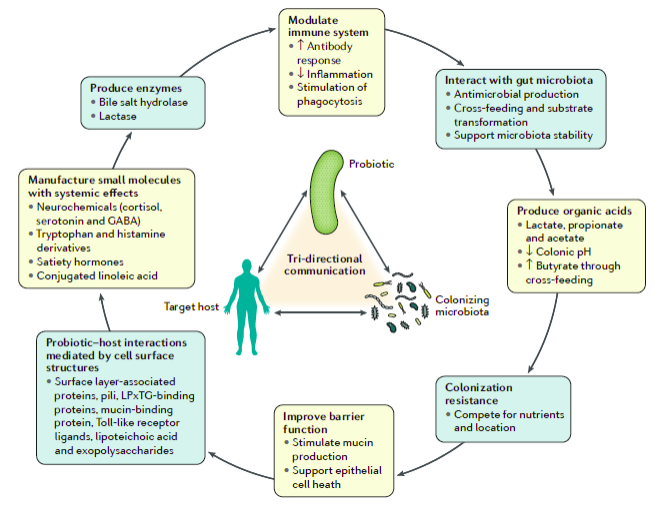
\includegraphics[width=0.8\textwidth]{Figures/probiotic_mechanisms.png}
    \caption{Proposed probiotic mechanisms \cite*{fig-pro_mech}}
    \label{fig:ProbioticMechanisms}
\end{figure}

\subsection{Synbiotics: Concept and Applications}
Synbiotics as a concept were first conceived in 1995. It is a combination of live microorganisms and prebiotics that together confer health benefits. There are two tupes of synbiotics, complementary and synergistic. Complementary synbiotics are when the prebiotic and probiotic are separate, while synergistic synbiotics are when the prebiotic and probiotic are combined \cite*{L6-Yeasts}.

\subsection{Postbiotics: A New Concept in Microbiome-Based Interventions}
Postbiotics are defined as preparations of inanimate microorganisms or their components that provide health benefits. This concept emphasizes the role of non-viable microbial products in health, including their potential effects beyond the gut. Furthermore it was emphasized in the lecture, that heat-treated fermented foods can also be considered postbiotics, highlighting their clinical relevance in some studies.

\section{02.10.24 - \textit{Bacillus} classification, physiology and use in fermented foods}
\subsection{Standard Methods for Describing Bacterial Taxa}
When characterizing bacterial taxa, various methods such as microscopic and macroscopic morphology, physiological and biochemical characteristics, and nucleic acid studies should be taken into account. When using multiple strains from diverse sources it is important to establish a comprehensive understanding of bacterial classification.

\subsection{Taxonomy and Classification of Bacillus Species}
\textit{Bacillus} is classified within the phylum \textit{Firmicutes}. It's a  diverse genus, which includes approximately 266 species. Key species in fermented foods include \textit{B. subtilis}, \textit{B. cereus}, and \textit{B. thuringiensis}. 

\subsection{Physiological Characteristics and Cell Morphology of Bacillus Species}
\textit{Bacillus} species are typically Gram-positive, rod-shaped bacteria that can thrive in aerobic or facultative anaerobic conditions. Their motility and presence in various environments, including fermented foods and the human gut, highlight their ecological significance and adaptability.

\subsection{Sporulation Structure and Process in Bacillus}
The sporulation process in \textit{Bacillus} is a survival mechanism induced by nutrient starvation, resulting in the formation of resilient endospores. These endospores are characterized by their protective structures and low water content, enabling them to withstand extreme environmental conditions.

\subsection{Biochemical Testing and Molecular Methods for Bacillus Identification}
Identification of \textit{Bacillus} species relies on a combination of biochemical tests and advanced molecular methods, such as DNA typing and 16S rRNA sequencing. Phenotypic test may have limitations in distinguishing closely related species, necessitating a multifaceted approach (both phenotypic and genotypic) to identification.

\subsection{Bacillus Species in Traditional Fermented Foods}
\textit{Bacillus} species are important in the production of traditional fermented foods, such as Natto and Soumbala. The fermentation processes, whether spontaneous or controlled, significantly influence the microbial community and the quality of the final product.

\subsection{Technological Properties and Applications of Bacillus in Food Fermentation}
The technological properties of \textit{Bacillus} species contribute to enhanced food fermentation through enzyme production (e.g. proteases, peptidases, amylases and glucosidases), which improves nutrient bioavailability and flavor. These properties also help reduce anti-nutritional factors, thereby increasing the overall nutritional value of fermented products.

\section{07.10.24 - Introduction to fermentation processes}
\subsection{Introduction to Fermentation Processes}
Fermentation is a crucial biological process that transforms sugars into alcohol or acids using microorganisms. Understanding fermentation processes is essential for producing various food products and improving their quality.




